\documentclass[border=4pt]{standalone}
\usepackage{pgfplots}
\usepgfplotslibrary{fillbetween}
\pgfplotsset{compat=1.18}

\begin{document}
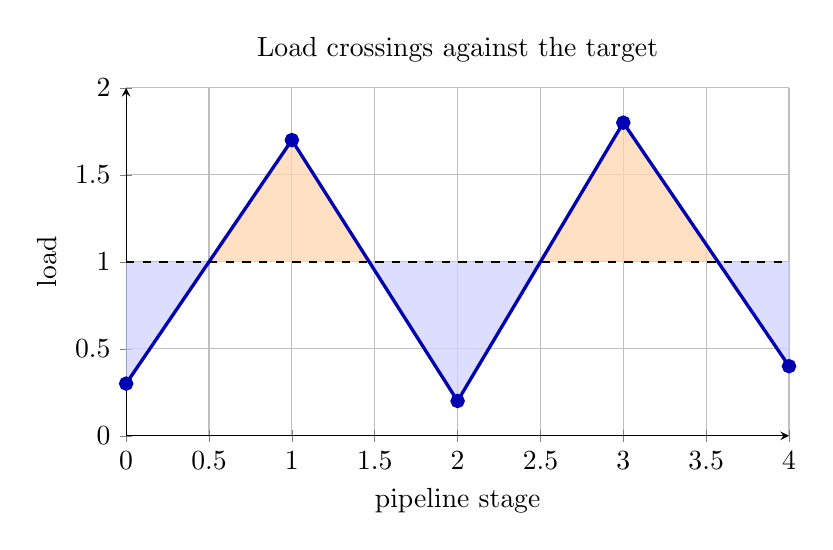
\begin{tikzpicture}
  \begin{axis}[
    width=10cm,
    height=6cm,
    xmin=0,
    xmax=4,
    ymin=0,
    ymax=2,
    axis lines=left,
    grid=major,
    xlabel={pipeline stage},
    ylabel={load},
    title={Load crossings against the target}
  ]
    \addplot[
      name path=load,
      blue!70!black,
      very thick,
      mark=*
    ] coordinates {
      (0,0.3) (1,1.7) (2,0.2) (3,1.8) (4,0.4)
    };
    \addplot[
      name path=target,
      black,
      thick,
      dashed
    ] coordinates {
      (0,1) (4,1)
    };
    \addplot[fill=blue!18,fill opacity=0.75] fill between[
      of=load and target,
      split,
      every even segment/.style={fill=blue!18},
      every odd segment/.style={fill=orange!32}
    ];
  \end{axis}
\end{tikzpicture}
\end{document}
